\chapter{DDD}

\section{Giới thiệu về thiết kế hướng miền (Domain Driven Design)}

% gioi_thieu_ve_thiet_ke_huong_mien_domain_driven_design}

\section{Cốt lõi của thiết kế hướng miền}

% Giới thiệu về các mẫu chiến lược và các mẫu kỹ thuật

% Thiết kế hướng miền cung cấp 2 loại mẫu:

\begin{itemize}

\item \emph{Các mẫu chiến lược (Strategic Patterns):} Phân chia một miền lớn và phức tạp thành các phần nhỏ hơn với ranh giới được xác định rõ ràng. Giúp phân chia một miền lớn hợp lý.

\item \emph{Các mẫu kỹ thuật (Tactical Patterns):} Hiện thực hóa các khái niệm và qui trình trong thành phần thành các thiết kế hệ thống phần mềm. Giúp hệ thống phù hợp với kinh doanh.

\end{itemize}

\begin{figure}[H]

\centering

\includegraphics[scale = 0.5]{pictures/cac_mau_chien_luoc_va_cac_mau_ky_thuat/main.drawio.png}

\caption{Tổng quan về Strategic Patterns và Tactical Patterns}

\end{figure}

% Thiết kế hướng miền cung cấp 2 loại mẫu:

\begin{itemize}

\item \emph{Các mẫu chiến lược (Strategic Patterns):} Phân chia một miền lớn và phức tạp thành các phần nhỏ hơn với ranh giới được xác định rõ ràng. Giúp phân chia một miền lớn hợp lý.

\item \emph{Các mẫu kỹ thuật (Tactical Patterns):} Hiện thực hóa các khái niệm và qui trình trong thành phần thành các thiết kế hệ thống phần mềm. Giúp hệ thống phù hợp với kinh doanh.

\end{itemize}

\begin{figure}[H]

\centering

\includegraphics[scale = 0.5]{pictures/cac_mau_chien_luoc_va_cac_mau_ky_thuat/main.drawio.png}

\caption{Tổng quan về Strategic Patterns và Tactical Patterns}

\end{figure}

% \subsection{Chi tiết về các mẫu chiến lược và các mẫu kỹ thuật}

\section{Các mẫu chiến lược của thiết kế hướng miền}

% \chapter{Các mẫu chiến lược}

% Các mẫu chiến lược phân tích nghiệp vụ kinh doanh sau đó đưa ra việc phân chia các thành phần và hiểu mối quan hệ của các thành phần đó. Từ đó, các mẫu chiến lược giúp xác định các thành phần quan trọng của hệ thống, đảm bảo kiến trúc phần mềm phản ánh đúng các yêu cầu kinh doanh. Từ việc phân chia hệ thống thành các thành phần nhỏ, chúng ta có thể tạo ra hệ thống mở rộng dễ dàng, phát triển linh hoạt theo nhu cầu kinh doanh.

Các mẫu chiến lược bao gồm:

\begin{itemize}

% các mục nhỏ ben dưới

% các mục nhỏ ben dưới

% các mục nhỏ ben dưới

% các mục nhỏ ben dưới

% các mục nhỏ ben dưới

% các mục nhỏ ben dưới

\item Muc1

\item Muc2

\item Muc1

\item Muc2

\item Muc1

\item Muc2

\item Muc1

\item Muc2

\end{itemize}

% nội dung trang lớn lên để hết giấy

% nội dung trang lớn lên để hết giấy

% nội dung trang lớn lên để hết giấy

% nội dung trang lớn lên để hết giấy

% nội dung trang lớn lên để hết giấy

\begin{figure}[H]

\centering

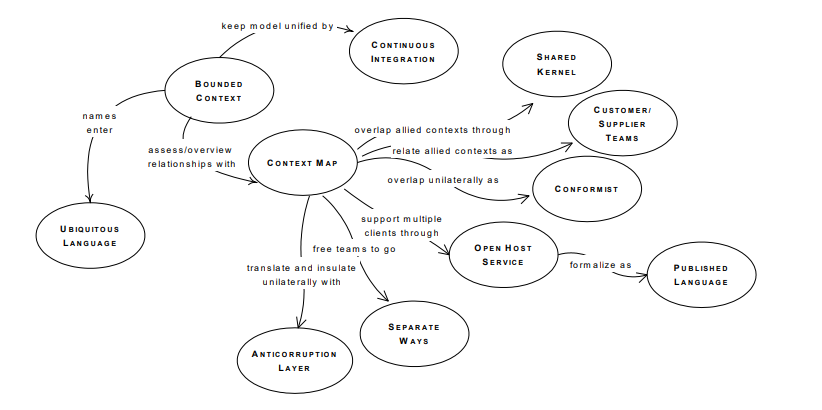
\includegraphics[scale = 0.9]{pictures/cac_mau_chien_luoc/temp.png}

\caption{Sơ đồ về các thành phần trong mô hình chiến lược}

\end{figure}

%!<! - - $ Vẽ lại sau: - - >

%!<! - - $ Vẽ lại sau: - - >

%!<! - - $ Vẽ lại sau: - - >

%!<! - - $ Vẽ lại sau: - - >

%!<! - - $ Vẽ lại sau: - - >

%!<! - - $ Vẽ lại sau: - - >

%!<! - - $ Vẽ lại sau: - - >

%!<! - - $ Vẽ lại sau: - - >

%!<! - - $ Vẽ lại sau: - - >

%!<! - - $ Vẽ lại sau: - - >



% \section{Miền phụ (Sub - Domain)}

% Một miền lớn được tạo thành từ nhiều \emph{miền phụ (Sub - Domain)}. Trong thực tế, một miền kinh doanh phức tạp không thể có một chuyên gia ngành có kiến thức về tất cả các miền phụ.

\begin{example} Trong miền thương mại điện tử lớn có thể có một số miền phụ sau:

\begin{itemize}

\item \textbf{Miền phụ quản lý hàng tồn kho:} liên quan đến việc quản lý sản phẩm trong kho hàng.

\item \textbf{Miền phụ quản lý khách hàng:} liên quan đến việc quản lý tài khoản khách hàng.

\item \textbf{Miền phụ vận chuyển:} liên quan đến việc quản lý việc vận chuyển giao hàng.

\end{itemize}

\end{example}



% \subsection{Phân loại các miền phụ}

% Trong thiết kế hướng miền, có ba loại miền phụ là:

\begin{itemize}

\item Miền phụ chung (Generic Subdomain)

\item Miền phụ cốt lõi (Core Subdomain)

\item Miền phụ hỗ trợ (Supporting Subdomain)

\end{itemize}

% \subsubsection{Miền phụ chung (Generic Subdomain)}

% Miền phụ chung cung cấp các giải pháp có sẵn mà doanh nghiệp có thể mua. Miền phụ chung có thể được tìm thấy trên nhiều ngành. Doanh nghiệp không thể đạt được bất kỳ lợi thế cạnh tranh nào so với đối thủ bằng cách thực hiện những điều khác biệt trong miền phụ chung.

\begin{example} Các miền phụ chung \textit{"quản lý nhân sự"} hay \textit{"quản lý cơ sở vật chất"} không tạo thêm bất kỳ giá trị khác biệt nào cho doanh nghiệp.

\end{example}



% \subsubsection{Miền phụ cốt lõi (Core Subdomain)}

% Miền phụ cốt lõi là phần quan trọng và có giá trị nhất của hệ thống. Miền phụ cốt lõi giúp phân biệt các doanh nghiệp và làm cho các doanh nghiệp có giá trị. Miền phụ cốt lõi tập trung vào mục tiêu và yêu cầu của khách hàng với doanh nghiệp, từ đó quyết định sự thành công của doanh nghiệp. Vì vậy, mỗi doanh nghiệp luôn tìm cách thực hiện những điều khác biệt trong các miền phụ cốt lõi này để đạt được lợi thế so với đối thủ cạnh tranh.

\begin{example} Trong miền thẻ tín dụng, miền phụ cốt lõi có thể là \textit{"phát hành thẻ"} chịu trách nhiệm về quá trình phát hành thẻ tín dụng cho khách hàng. Miền phụ cốt lõi này bao gồm các nhiệm vụ như: thu thập thông tin khách hàng, thực hiện kiểm tra tín dụng, kích hoạt thẻ, \dots

\end{example}

% \subsubsection{Miền phụ hỗ trợ (Supporting Subdomain)}

% Các miền phụ cốt lõi phụ thuộc vào các miền phụ hỗ trợ. Miền phụ hỗ trợ cung cấp các dịch vụ để miền phụ cốt lõi hoạt động hiệu quả. Tuy nhiên, miền phụ hỗ trợ không đòi hỏi mức độ phức tạp cao về logic nghiệp vụ.

\begin{example} Trong nhiều phần mềm, miền phụ hỗ trợ \textit{"xác thực người dùng"} OAuth 2.0 của Facebook hoặc Google hỗ trợ cho miền phụ cốt lõi hoạt động hiệu quả.

\end{example}
 
% \subsection{Cách xác định các miền phụ}

% Các miền phụ cốt lõi, hỗ trợ và chung có thể khác nhau đối với các doanh nghiệp hoạt động trong cùng một miền. Vì các miền phụ được xác định tùy theo nhu cầu kinh doanh và bối cảnh cụ thể của mỗi tổ chức.

\subsubsection{Mô tả cách xác định các miền phụ}

\begin{enumerate}

\item Bắt đầu bằng cách xem xét nghiệp vụ kinh doanh.

\item Nếu có sẵn giải pháp đã biết thì có khả năng là miền phụ chung. Ngược lại, chúng ta kiểm tra nghiệp vụ kinh doanh đó có thêm giá trị kinh doanh nào hay không?

\item Nếu không có giá trị kinh doanh thì chúng ta kiểm tra xem các miền phụ cốt lõi có phụ thuộc vào miền phụ này hay không? Nếu có thì có khả năng là miền phụ hỗ trợ. Nếu không thì đó là miền phụ chung.

\item Nếu miền phụ có tiềm năng bổ sung một số giá trị kinh doanh thì bước kiểm tra tiếp theo là xem liệu miền doanh nghiệp có độ phức tạp cao hay không?

\item Nếu miền doanh nghiệp không có độ phức tạp cao thì có khả năng là miền phụ hỗ trợ. Ngược lại thì nó có khả năng là miền phụ cốt lõi.

\end{enumerate}

\begin{figure}[h]

\centering

\includegraphics[scale = 0.5]{pictures/cach_xac_dinh_cac_mien_phu/main.drawio.png}

\caption{Sơ đồ xác định các miền phụ}

\end{figure}



% \subsection{Áp dụng phân loại miền phụ trong đồ án này}

% % %!<! - - Hướng dẫn: 5/3 - - >

% %!<! - - Hướng dẫn: 5/3 - - >

% %!<! - - Hướng dẫn: 5/3 - - >

% %!<! - - Hướng dẫn: 5/3 - - >

% %!<! - - Hướng dẫn: 5/3 - - >

% %!<! - - Hướng dẫn: 5/3 - - >

% %!<! - - Hướng dẫn: 5/3 - - >

% %!<! - - Hướng dẫn: 5/3 - - >

% %!<! - - Hướng dẫn: 5/3 - - >

% %!<! - - Hướng dẫn: 5/3 - - >

% %!<! - - Hướng dẫn: 5/3 - - >

% %!<! - - Hướng dẫn: 5/3 - - >

% %!<! - - Hướng dẫn: 5/3 - - >

% %!<! - - Hướng dẫn: 5/3 - - >

% %!<! - - Hướng dẫn: 5/3 - - >

% %!<! - - Hướng dẫn: 5/3 - - >

% ChatGPT?

% Ứng dụng thiết kế hướng miền với hóa đơn điện tử thì miền phụ hỗ trợ có thể là gì?

\subsubsection{Áp dụng phân loại miền phụ trong đồ án này}

\subsubsection{Áp dụng phân loại miền phụ trong đồ án này}

\subsubsection{Áp dụng phân loại miền phụ trong đồ án này}

\subsubsection{Áp dụng phân loại miền phụ trong đồ án này}

\subsubsection{Áp dụng phân loại miền phụ trong đồ án này}

\subsubsection{Áp dụng phân loại miền phụ trong đồ án này}

\subsubsection{Áp dụng phân loại miền phụ trong đồ án này}

\subsubsection{Áp dụng phân loại miền phụ trong đồ án này}

\subsubsection{Áp dụng phân loại miền phụ trong đồ án này}

\subsubsection{Áp dụng phân loại miền phụ trong đồ án này}

\subsubsection{Áp dụng phân loại miền phụ trong đồ án này}

\subsubsection{Áp dụng phân loại miền phụ trong đồ án này}

\subsubsection{Áp dụng phân loại miền phụ trong đồ án này}



\section{Các mẫu kỹ thuật của thiết kế hướng miền}

\section{DDD}

\section{DDD}

\section{DDD}

\section{DDD}

\section{DDD}

